\documentclass{beamer}

\usepackage{hyperref}
\usepackage[subpreambles=true]{standalone}
\usepackage{tikz}
\usetikzlibrary{positioning, fit}

%****************************************************************
% Some settings
%****************************************************************
\usecolortheme{beaver}
\usefonttheme{default}
\usetheme{CambridgeUS}

%\graphicspath{{figures/}}

\setbeamertemplate{navigation symbols}{}

%****************************************************************
% Define color
%****************************************************************
\definecolor{MITred}{RGB}{163,31,52}
\definecolor{MITgray}{RGB}{138,139,140}
\definecolor{MITlightgray}{RGB}{194,192,191}

%****************************************************************
% Modify footline & headline
%****************************************************************
%gets rid of bottom navigation bars
\setbeamertemplate{footline}[frame number]{}

%gets rid of header
\setbeamertemplate{headline}{}

%****************************************************************
% Modify title
%****************************************************************
\setbeamertemplate{title page}[default][colsep=-4bp,rounded=true]

%****************************************************************
% Modify table of contents
%****************************************************************
\setbeamertemplate{section in toc}{{\color{MITred}%
  \MakeUppercase{\romannumeral \inserttocsectionnumber}.}%
~\inserttocsection}
\setbeamertemplate{subsection in toc}{\hspace{1.2em}{\color{MITred}%
{\tiny $\blacksquare$}}~\inserttocsubsection \par}
\setbeamertemplate{subsubsection in toc}{\hspace{2.4em}%
{\color{MITred}{\tiny $\square$}}~\inserttocsubsection \par}

%****************************************************************
% Modify frame
%****************************************************************
\setbeamercolor{frametitle}{fg=MITred}
\setbeamertemplate{blocks}[rounded][shadow=false]
\setbeamercolor{block title}{fg=MITred}

%****************************************************************
% Modify numerate & itemize bullet
%****************************************************************
\setbeamercolor{enumerate item}{fg=MITred}
\setbeamercolor{enumerate subitem}{fg=MITred}
\setbeamercolor{enumerate subsubitem}{fg=MITred}
\setbeamertemplate{enumerate items}[default]

\setbeamercolor{itemize item}{fg=MITred}
\setbeamercolor{itemize subitem}{fg=MITred}
\setbeamercolor{itemize subsubitem}{fg=MITred}
\setbeamertemplate{itemize item}[triangle]
\setbeamertemplate{itemize subitem}{$  riangleright$}
\setbeamertemplate{itemize subsubitem}{$ullet$}

%****************************************************************
% Some definitions
%****************************************************************
\providecommand{\figurepath}{figures}
\providecommand{\datapath}{data}

\standaloneconfig{build={command=%
{\latex\space\latexoptions\space\quote\string\newcommand{\string\figurepath}%
{\figurepath}\string\newcommand{\string\datapath}{\datapath}\string\input{\file}\quote}}}

%****************************************************************
% Title
%****************************************************************

%****************************************************************
% Begin document
%****************************************************************
\begin{document}
\begin{frame}
  \frametitle{Statistical inverse problems governed by PDEs}
  \begin{columns}
    \begin{column}{0.55\textwidth}
      \vspace{-0.5cm}
      \begin{figure}
        \centering
        \resizebox{\columnwidth}{!}
        {
          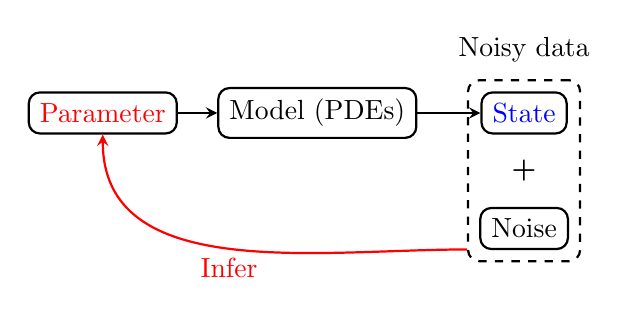
\begin{tikzpicture}[>=stealth, mybox/.style={thick, rounded corners, inner sep=4}]
            \node [mybox, draw=black] (parameter) {\color{red} Parameter};
            \node [mybox, draw=black, right=0.5cm of parameter] (model) {Model (PDEs)};
            \node [mybox, draw=black, right=0.8cm of model] (state) {\color{blue} State};
            \node [below=0.2cm of state] (plus) {\textbf{+}};
            \node [mybox, draw=black, below=0.2cm of plus] (noise) {Noise};

            \node [mybox, draw=black, dashed, fit={(state) (noise)}] (noisy_data) {};

            \node [above=0.1cm of noisy_data] {Noisy data};

            \path [->, thick] (parameter.east) edge (model.west)
            (model.east) edge (state.west)
            ([yshift=-1cm] noisy_data.west) edge[out=180, in=-90, red] node[below]
            {Infer} (parameter.south);

            % \node [very thick, draw=black, fit={(parameter) (model) (noisy_data)}] () {};
          \end{tikzpicture}
        }
      \end{figure}

      Goal:
      \begin{itemize}
        \item infer unknown {\color{red} parameters} from limited noisy
          {\color{blue} state} observations through governing partial
          differential equation (PDE) models,
        \item quantify uncertainties in the parameter inference.
      \end{itemize}

    \end{column}
    \begin{column}{0.45\textwidth}
      \begin{figure}
        \centering
        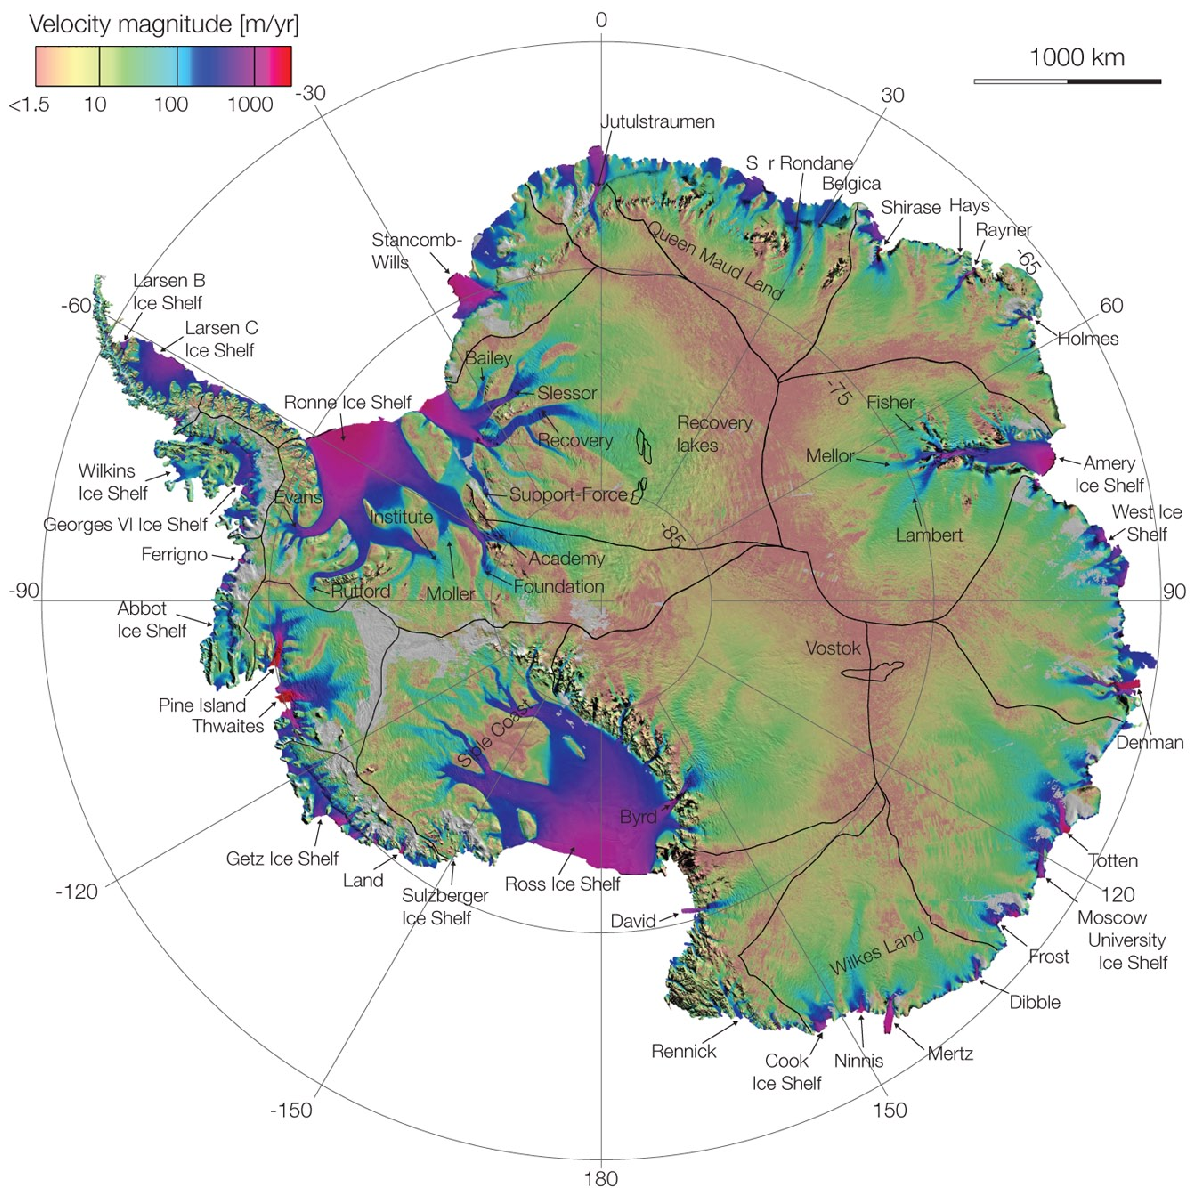
\includegraphics[width=0.5\columnwidth]{figures/ScienceRignot-crop.pdf}
      \end{figure}
      \vspace{-0.5cm}
      \begin{center}
        {\tiny Observed surface velocity field (Rignot et. al, 2011)}
      \end{center}
      \begin{figure}
        \centering
        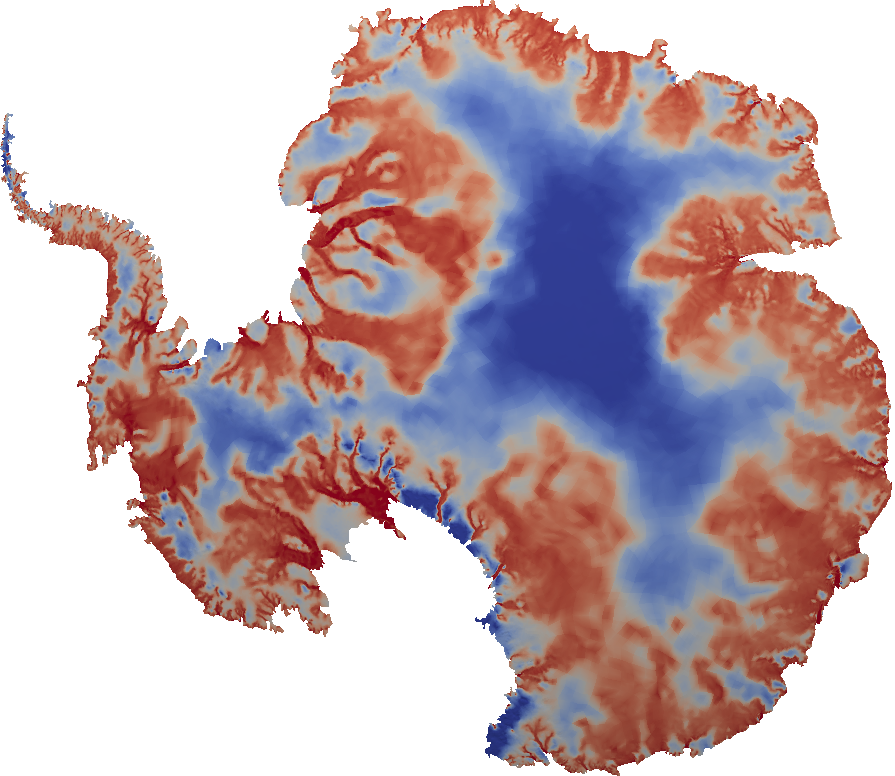
\includegraphics[width=0.4\columnwidth]{figures/antarctica_beta.png}
      \end{figure}
      \begin{center}
        {\tiny Inferred basal friction parameter field (Isaac et. al, 2015))}
      \end{center}
    \end{column}
  \end{columns}
\end{frame}

\begin{frame}
  \frametitle{Bayesian framework for the inverse problem}

  \begin{center}
    \includestandalone[mode=buildnew, width=\textwidth]{tikz/bayesian_diagram}
  \end{center}
\end{frame}

\begin{frame}
  \frametitle{Solution of Bayesian inverse problems governed by PDEs}

  \begin{block}{Markov Chain Monte Carlo (MCMC) method:}
    \begin{itemize}
      \item An effective and systematic way to characterize the posterior
      \item Generates samples from the posterior, which are then used in Monte
        Carlo approximations of quantity of interest $Q$
      \item For example, the posterior expectation of quantity of interest $Q$ is estimated as
        \vspace{-0.5cm}
        $$
          \mathbb{E}[Q] = \int Q(\mathbf{\textcolor{red}{m}}) \pi_\text{post} (\mathbf{\textcolor{red}{m}} |
          \mathbf{d}) d \mathbf{\textcolor{red}{m}}
          \approx \frac{1}{n_s} \sum_{i}^{n_s} Q(\textcolor{red}{\mathbf{m}_i})
        $$
    \end{itemize}
  \end{block}

  \begin{block}{MCMC method is computationally prohibitive (for
    high-dimensional parameter and state spaces after discretization):}
    \begin{itemize}
      \item Requires repeated evaluations of expensive-to-solve large-scale PDE models
      \item Samples are autocorrelated $\rightarrow$ poor estimation of the
        posterior
      \item Curse of dimensionality: dimension of parameter $\mathbf{m}$ $\uparrow$
        $\rightarrow$ sampling efficiency $\downarrow$
    \end{itemize}
  \end{block}
\end{frame}

\begin{frame}
  \frametitle{Jointly-reduced Bayesian inversion approach}
  \begin{center}
    % \includestandalone[mode=buildnew, width=\textwidth]{tikz/summary_reduced_bayes}
    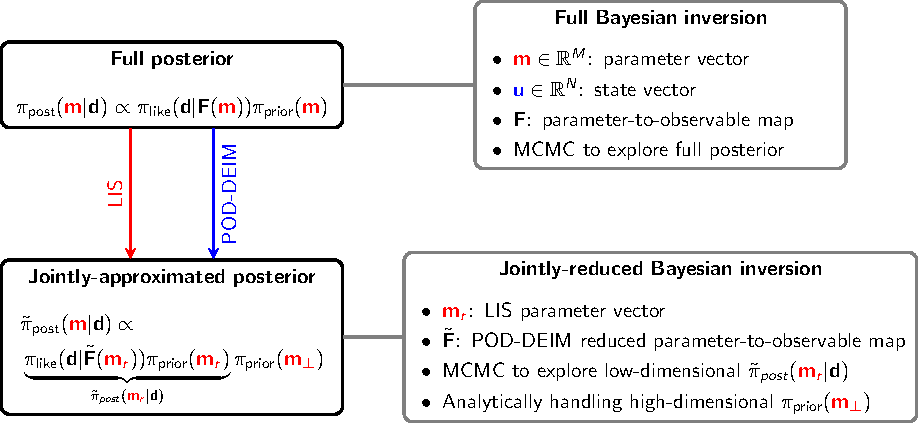
\includegraphics[width=\columnwidth]{tikz/summary_reduced_bayes.pdf}
  \end{center}

  \begin{itemize}
    \item Parameter dimension reduction by likelihood-informed-subspace (LIS)
    \item State dimension reduction by Proper orthogonal decomposition (POD) with
      discrete empirical interpolation method (DEIM)
  \end{itemize}

  \vspace{0.3cm}

  \tiny
  \begin{itemize}
    \item [] Details in: K. Kim, B. Peherstorfer, T. Cui, Y. Marzouk, K.
      Willcox, O. Ghattas, and N. Petra. “Joint Parameter and Model Dimension
      Reduction for Bayesian Inverse Problems with Application to a Nonlinear
      Stokes Ice Sheet Flow”. In preparation.
  \end{itemize}
\end{frame}

\begin{frame}
  \frametitle{Jointly-reduced Bayesian inversion approach}
  \framesubtitle{Example -- a 2D rectangular ice sheet model problem}
  \begin{center}
    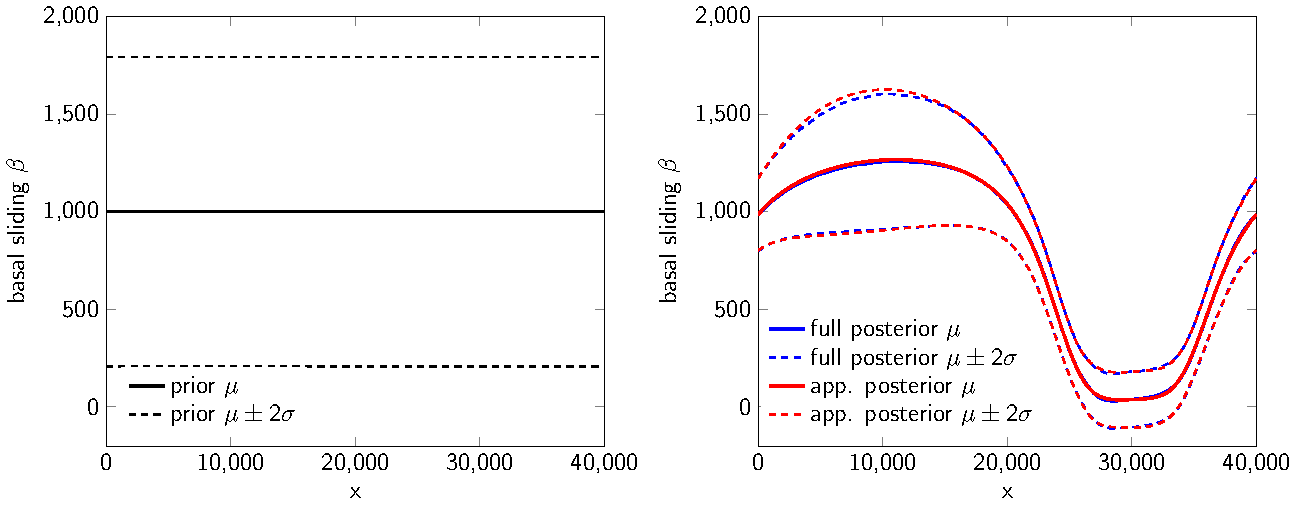
\includegraphics[width=\columnwidth]{figures/basal_estimates.pdf}
  \end{center}

  \scriptsize
  \begin{itemize}
    \item \textcolor{blue}{Full posterior}: 120 dim. parameters + 4,920 dim. states
    \item \textcolor{red}{Jointly approximated posterior}: 10 dim. parameters + 30 dim. states (200 dim. DEIM)
    \item 15 horizontal velocity observations on the right half side of the top boundary
    \item 60,000 samples from the full posterior, 15,000 samples from the jointly-reduced posterior
    \item H-pCN (Hessian informed Crank-Nicolson) MCMC method is used to sample
  \end{itemize}

  \vspace{0.2cm}

  \tiny
  \begin{itemize}
    \item[] Details in: K. Kim, U. Villa, M. Parno, N. Petra, Y. Marzouk, and
      O. Ghattas.. “hIPPYlib-MUQ: Scalable Markov chain Monte Carlo sampling
      methods for large-scale Bayesian inverse problems governed by PDEs”. To
      be submitted. Submitted. (\url{https://github.com/hippylib/hippylib2muq})

  \end{itemize}
  
\end{frame}

\end{document}
